\documentclass{article}
\usepackage[utf8]{inputenc}
\usepackage[margin = 0.8in]{geometry}
\usepackage{graphicx}
\usepackage{amsmath, amssymb}
\usepackage{subcaption}
\usepackage{multirow}
\usepackage{mathtools}
\usepackage{float}
\usepackage[linesnumbered,ruled]{algorithm2e}

\title{RBE595 - Midterm}
\author{Keith Chester}
\date{Due date: March 26, 2023}

\begin{document}
\maketitle

\section*{Problem 1}

In this question we are presented with two random variables with provided distributions $p={0.2, 0.2, 0.2, 0.2, 0.1, 0.1}$ and $q={0.75, 0.0625, 0.0625, 0.0625, 0.0625}$.

\subsection*{1.1}
\textit{Calculate the entropy for each variable}

To do this, we use the equation:

\begin{equation}
    H(p) = - \sum_{i=1}^{n} p_i \log_2 p_i
\end{equation}

...where $n$ is the number of values within the distribution. Thus we can

\begin{equation}
    H(p) = - \sum_{i=1}^{6} p_i \log p_i \
    = - (0.2 \log_2 0.2 + 0.2 \log_2 0.2 + 0.2 \log_2 0.2 + 0.2 \log_2 0.2 + 0.1 \log_2 0.1 + 0.1 \log_2 0.1) \
\end{equation}
\begin{equation}
    = - (4*(0.2 *-2.32193) + 2 *( 0.1 * -3.32193) ) = 2.52193
\end{equation}

...and then for the next distribution:

\begin{equation}
    H(q) = - \sum_{i=1}^{5} q_i \log_2 q_i \
    = - (0.75 \log_2 0.75 + 0.0625 \log_2 0.0625 + 0.0625 \log_2 0.0625 + 0.0625 \log_2 0.0625 + 0.0625 \log_2 0.0625)
\end{equation}

\begin{equation}
    = - ( (0.75 * -0.415) + 4*(0.0625 * -4) ) = 1.31125
\end{equation}

...thus $p$ has $2.522$ bits of entropy, and $q$ has $1.311$ bits of entropy.

\subsection*{1.2}

\textit{Intuitively how can you tell which variable has a higher entropy without calculating the entropy numerically? What does higher entropy mean?}

A random variable with high entropy means that the distribution/outcome is more uncertain/unpredictable. It's probability function is more spread out or has a wider ranger of possible values.Since $q$ has single value it is skewed towards, we would suspect that $p$ would have greater entropy; our calculations confirm this.


\section*{Problem 2}

\textit{Which equation correctly relates $v*$ to $q*$? Draw the corresponding backup-diagram and explain.}

\begin{itemize}
    \item \textbf{A} - $v_*(s) = \sum_{r,s} \pi(a|s)p(s', r|s,a)[r+\gamma q_* (s')]$
    \item \textbf{B} - $v_*(s) = max_a q_*(s|a)$
    \item \textbf{C} - $v_*(s)= max_a \sum_{r,s} p(s', r|s,a)[r+\gamma q_*(s',a)]$
    \item \textbf{D} - $v_*(s) = max_a \sum_{r,s'} p(s',r|s, a)[r+\gamma v_*(s')] $
    \item \textbf{E} - None of the above
    \item \textbf{F} - B and D
\end{itemize}

Answer:

\textbf{F} - both \textbf{B} and \textbf{D}

You can see the backup diagrams for each drawn in Figure 1.

\begin{figure}
    \centering
    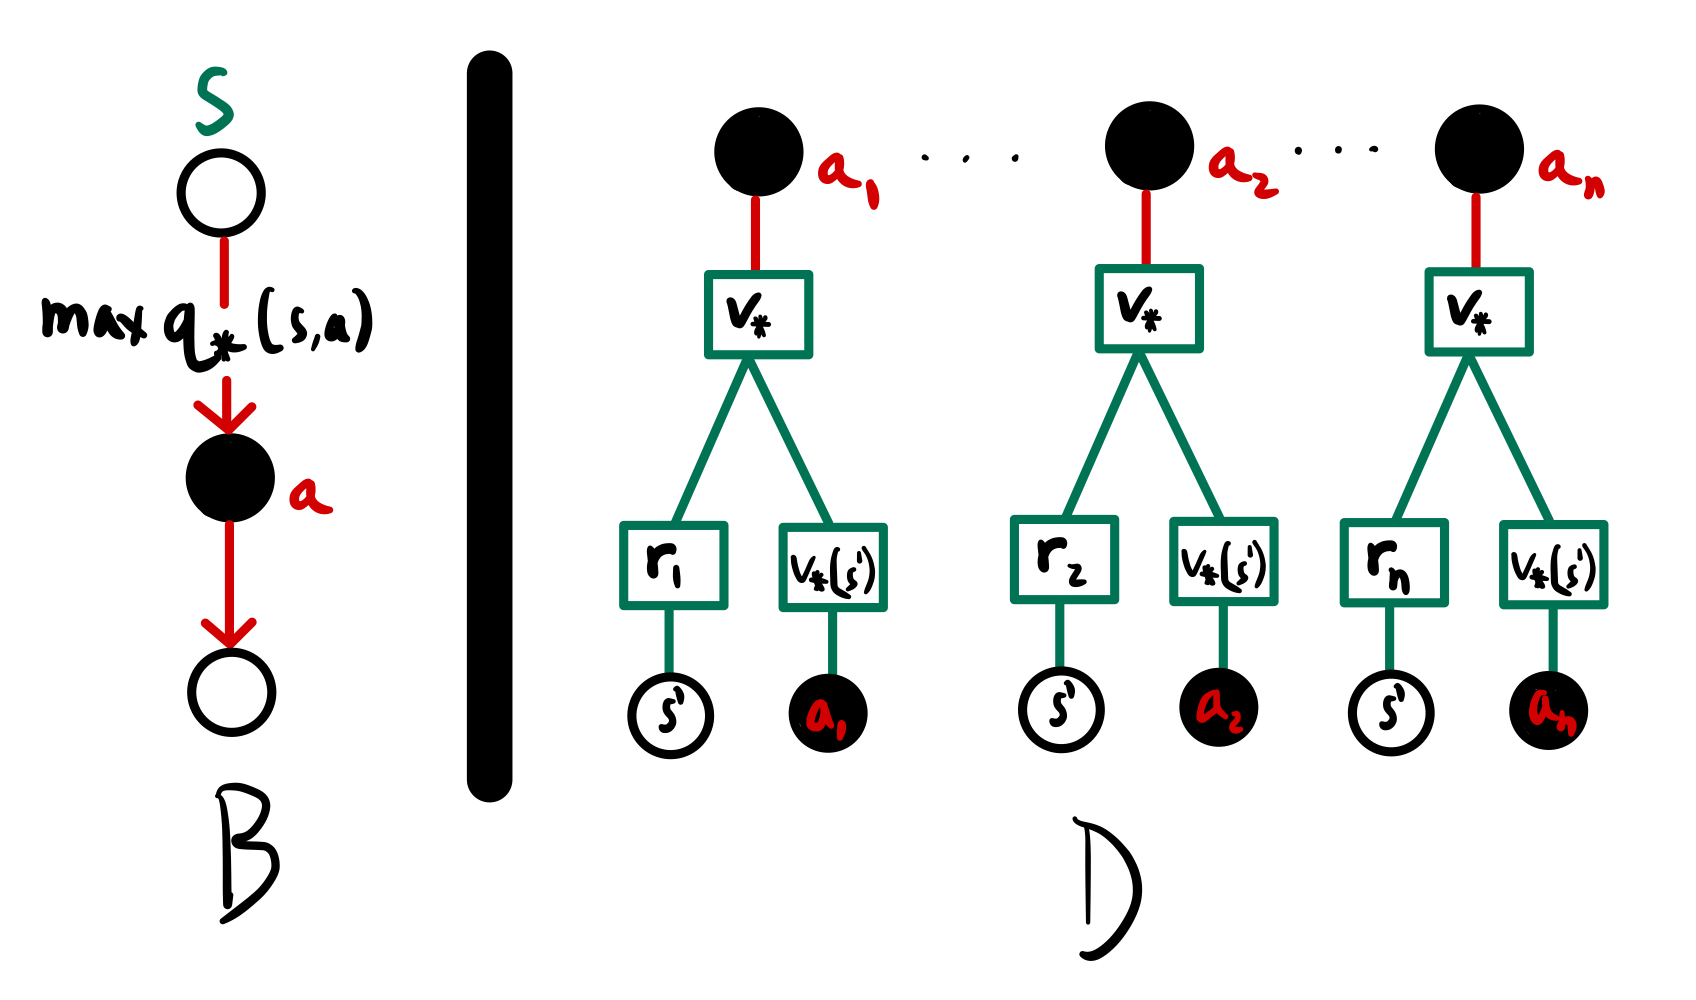
\includegraphics[width=.8\linewidth]{imgs/midterm.backup.diagram.png}
    \caption{Backup diagram for B and D}
\end{figure}

\textbf{Reasoning:}

\begin{itemize}
    \item \textbf{A} - This is incorrect as it uses $q_*$ in place of $v_*$ in the backup equation.
    \item \textbf{B} - This directly computes the optimal state value via its greedy action of calculating the maximum of all actions and their resulting action values
    \item \textbf{C} - This is incorrect as it computes the expected value of the next state using the current state/action pair - it should use the next state/action pair $s',a$
    \item \textbf{D} - The definition of $q_*(s,a)$ as taking the expected return of state $s$ with action $a$ and taking the optimal thereafter; therefore we can take the maximum of all actions \textbf{D} returns and get the Bellman Equation.
    \item \textbf{E} -Since B and D is right, this is eliminated
    \item \textbf{F} - B and D are correct, so we choose this.
\end{itemize}

\section*{Problem 3}

\textit{Consider a vehicle with 4 actions (left,right,up, down). There’s no uncertainty in the outcome ofthe action (i.e. when left is commanded, the left state is achived). The actions that cause the vehicle outside the grid, leave the state unchanged. The reward for all transition is -1 except when the goal is reached where the reward is zero. Discount factor $\gamma = 1$}

\textit{Figure 2 shows the name of the states and figure on the right shows the state-value $V(s)$, for each state under a uniform random policy}

\begin{figure}
    \centering
    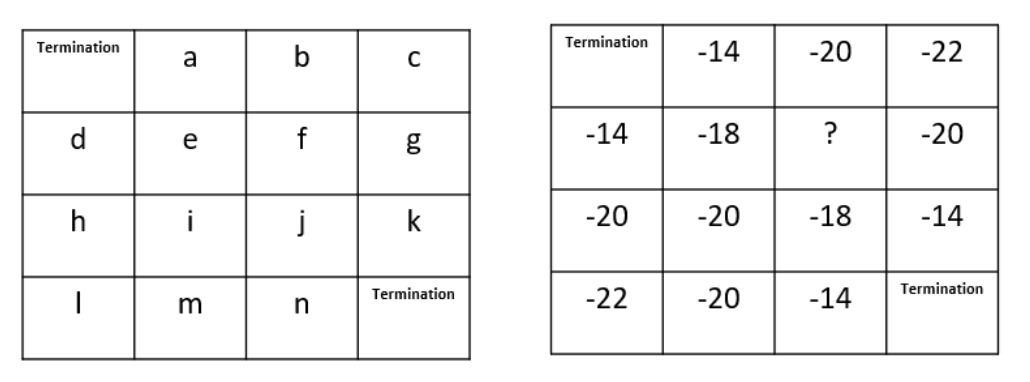
\includegraphics[width=.8\linewidth]{imgs/midterm.3.png}
    \caption{Problem 3: States and $V(s)$}
\end{figure}

\subsection*{3.1}

\textit{What is $q(k, \downarrow)$?}

\begin{equation}
    q(k, \downarrow) = r + \gamma V(k) = -1 + 1 * -14 = -15
\end{equation}



\subsection*{3.2}

\textit{What is $q(g, \downarrow)$?}

\begin{equation}
    q(k, \downarrow) = r + \gamma V(g) = -1 + 1 * -20 = -21
\end{equation}



\subsection*{3.3}

\textit{What is $V(f)$?}

...where $p(s)$ is the probability of choosing a given state $s'$, which for our initial calculation we will use uniform probability or $\frac{1}{4}$.

\begin{equation}
    V(s) = \frac{1}{4}(-1 + \gamma * V(b)) + \frac{1}{4}(-1 + \gamma * V(e)) + \frac{1}{4}(-1 + \gamma * V(g)) + \frac{1}{4}(-1 + \gamma * V(j))
\end{equation}

\begin{eqnarray}
    V(s) = \frac{1}{4}(-1 + 1 * -20) + \frac{1}{4}(-1 + 1 * -18) + \frac{1}{4}(-1 + 1 * -20) + \frac{1}{4}(-1 + 1 * -18)
\end{eqnarray}

\begin{equation}
    V(s) = \frac{-21}{4} + \frac{-19}{4} + \frac{-21}{4} + \frac{-19}{4} = \frac{-80}{4} = -20
\end{equation}


\section*{Problem 4}

\textit{Consider the state-action interaction in Figure 3. The $q(s,a)$ written next to each action (left and right) is the initial estimate.}

\begin{figure}
    \centering
    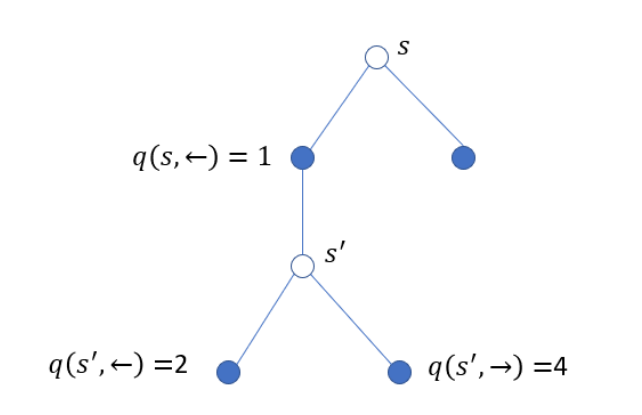
\includegraphics[width=.8\linewidth]{imgs/midterm.4.1.png}
    \caption{Problem 4: State-Interaction Tree}
\end{figure}

\textit{Consider a discount factor $\gamma = 0.5$ and learning rate $\alpha=0.1$, and a reward transition of $r=1$}

\subsection*{4.1}
\textit{What is the target value as well as updated value of $q(s,\leftarrow)$ using SARSA algorithm if the action at $s'$ was the left action.}

The update rule:
\begin{equation}
    q(s,a) \leftarrow q(s,a) + \alpha [R + \gamma q(s_{t+1},a) - Q(s,a)]
\end{equation}

...and the target value is:

\begin{equation}
    R_{t+1} + \gamma Q(s_{t+1}, a)
\end{equation}

So first we calculate target value:

\begin{equation}
    = 1 + 0.5 * 2 = 2
\end{equation}

...and then applying for the update value:

\begin{equation}
    q(s,a) \leftarrow 1 + 0.1 * (2 - 1) = 1.1
\end{equation}

\subsection*{4.2}

\textit{ What is the target value as well as updated value of $q(s, \leftarrow)$ using SARSA algorithm if the action at $s'$ was the right action.}

Target value:
\begin{equation}
    = 1 + 0.5 * 4 = 3
\end{equation}

Update value:
\begin{equation}
    q(s,a) \leftarrow 1 + 0.1 * (3 - 1) = 1.2
\end{equation}

\subsection*{4.3}

\textit{Assume that the action at $s'$ has a distribution in such a way that it is $30$ percent left action and $70$ percent right action. What is the expected SARSA target value and as well expected value of $q(s,\leftarrow$) under SARSA algorithm?}

The target value of Expected SARSA is:

\begin{equation}
    R_{t+1} + \gamma \sum_a \pi (a|s_{t+1})q(s_{t+1}, a)
\end{equation}

Target value:
\begin{equation}
    = 1 + 0.5 * ( 0.30 * 2 + 0.70 + 4 ) = 2.7
\end{equation}

Update value:
\begin{equation}
    q(s,a) \leftarrow 1 + 0.1 * (2.7 - 1) = 1.17
\end{equation}

\subsection*{4.4}

\textit{What is the target value as well as updated value of $q(s,\leftarrow)$ using Q-learning algorithm.}

Our target value formula is:

\begin{equation}
    R_{t+1} + \gamma max_a q(s_{t+1}, a)
\end{equation}

...and our update value is:

\begin{equation}
    q(s, a) \leftarrow q(s, a) + \alpha \left[r_{t+1} + \gamma \max_{a} Q(s_{t+1}, a) - Q(s, a)\right]
\end{equation}

So our target value is:

\begin{equation}
    1 + 0.5 * 4 = 3
\end{equation}

...and our update value is:

\begin{equation}
    q(s,a) \leftarrow 1 + 0.1 * (3 - 1) = 1.2
\end{equation}

\subsection*{4.5}

\textit{Does the distribution of the action at s' have an effect on the Q-learning target value?}

Yes, it does have an effect. The Q-learning target involves taking max of an action value over all possible states for $s'$, which in turn depends upon the distribution/probabilities of choosing actions in that state.

\subsection*{4.6}
\textit{Consider now we have another batch of initial estimates for the action-values. We call then $q'(s,a)$. They are shown in the diagram in Figure 4 in green color.}

\begin{figure}
    \centering
    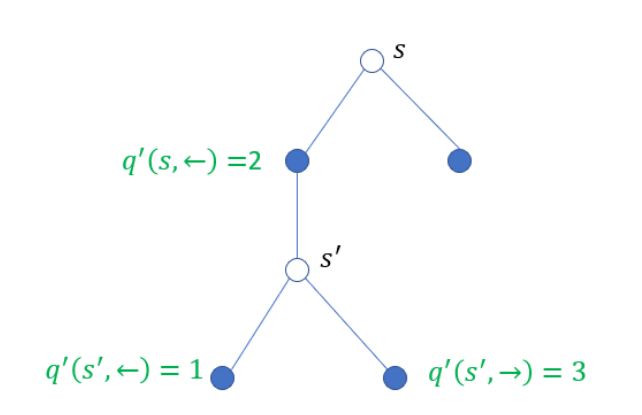
\includegraphics[width=.8\linewidth]{imgs/midterm.4.2.png}
    \caption{Problem 4: State-Interaction Tree Part 2}
\end{figure}

\textit{What is the updated value of $q(s, \leftarrow)$ using double-Q learning algorithm? (You need to use both green and black initial estimates)}

\begin{equation}
    q_{1}(s, a) \leftarrow q_{1}(s, a) + \alpha \bigl[r_{t+1} + \gamma q_{2}(s_{t+1}, \arg\max_{a} q_{1}(s_{t+1},a)) - q_{1}(s, a) \bigr]
\end{equation}
\begin{equation}
    q_{2}(s, a) \leftarrow q_{2}(s, a) + \alpha \bigl[r_{t+1} + \gamma q_{1}(s_{t+1}, \arg\max_{a} q_{2}(s_{t+1},a))- q_{2}(s, a) \bigr]
\end{equation}

So for this problem we look at $q_1(s,\leftarrow)$:

\begin{equation}
    q_1(s,a) \leftarrow 1 + 0.1 * (1 + (0.5* 3) - 1  ) = 1.15
\end{equation}

\subsection*{4.7}

\textit{What is the updated value of $q'(s,\leftarrow)$ using double-Q learning algorithm? (You need to use both green and black initial estimates)}

For $q'(s,\leftarrow)$ we use the $q_2(s,\leftarrow)$ calculation:

\begin{equation}
    q_2(s'a) \leftarrow 2 + 0.1 * (1 + (0.5 * 4) - 2) = 2.1
\end{equation}


\section*{Problem 5}

\textit{As we discussed, n-step off-policy return via bootstrapping can be written as:}

\begin{equation}
    G_{t:h} = p_t(R_{t+1} + \gamma G_{t+1:h})
\end{equation}

\textit{where $p=\frac{\pi(A_t|S_t)}{b(A_t|S_t)}$ is the importance sampling ratio between target and behavior policy.}

\textit{Using control variates, the return can be written as:}

\begin{equation}
    G_{t:h} = p_t(R_{t+1}+\gamma G_{t+1:h}) + (1-p_t) V_{h-1} (S_t)
\end{equation}

\textit{Prove that introducing the control variates in equation (2) does not add any bias to the original return (i.e. equation (1)) in expectation.}


We start with our original equation as instructed...
\begin{equation}
    G_{t:h} = p_t(R_{t+1} + \gamma G_{t+1:h})
\end{equation}

...then add in the control variate.
\begin{equation}
    G_{t:h} = p_t(R_{t+1}+\gamma G_{t+1:h}) + (1-p_t) V_{h-1} (S_t)
\end{equation}

We take the expected value of the probability of each element.
\begin{equation}
    \mathbb{E}[G_{t:h}] = \mathbb{E}[p_t(R_{t+1} + \gamma G_{t+1:h})] + \mathbb{E}[(1-p_t) V_{h-1} (S_t)]
\end{equation}

We simplify by realizing that $p_t$ is the only bit dealing with probability and isolated the expected value to that piece.
\begin{equation}
    \mathbb{E}[G_{t:h}] = \mathbb{E}[p_t(R_{t+1} + \gamma G_{t+1:h})] + (1-\mathbb{E}[p_t]) V_{h-1} (S_t)
\end{equation}

...using the law of total expectations, we can then make the following change, as $\mathbb{E}[p_t(R_{t+1} + \gamma G_{t+1:h})] = \mathbb{E}[\mathbb{E}[p_t(R_{t+1} + \gamma G_{t+1:h})|S_t, A_t]]$
\begin{equation}
    \mathbb{E}[G_{t:h}] = \mathbb{E}[\mathbb{E}[p_t(R_{t+1} + \gamma G_{t+1:h})|S_t,A_t]] + (1-\mathbb{E}[p_t]) V_{h-1} (S_t)
\end{equation}

We can use the definition of expected value to convert the inner expectation of the first term to the expected value of the given expression conditioned on the state-action pair...
\begin{equation}
    \mathbb{E}[G_{t:h}] = \mathbb{E}[\frac{\pi(A_t|S_t)}{b(A_t|S_t)}(R_{t+1} + \gamma \mathbb{E}[G_{t+1:h}|S_{t+1}])] + (1-\mathbb{E}[p_t]) V_{h-1} (S_t)
\end{equation}

\begin{equation}
    \mathbb{E}[G_{t:h}] = \sum_{a_t}\frac{\pi(a_t|S_t)}{b(a_t|S_t)}\sum_{r_{t+1},s_{t+1}}p(r_{t+1},s_{t+1}|S_t,a_t)[r_{t+1} + \gamma \mathbb{E}[G_{t+1:h}|S_{t+1}]]
\end{equation}

\begin{equation}
    \mathbb{E}[G_{t:h}] = \sum_{a_t}\pi(a_t|S_t)\sum_{r_{t+1},s_{t+1}}\frac{p(r_{t+1},s_{t+1}|S_t,a_t)}{b(a_t|S_t)}[r_{t+1} + \gamma \mathbb{E}[G_{t+1:h}|S_{t+1}]]
\end{equation}

Here we see that the expected value of the return with control variates is equivalent to the expected value of the return without the control variates because our last term ends up going to zero. Because of this, we can expect $p_t$ to go to 1:

\begin{equation}
    \mathbb{E}[p_t] = \mathbb{E}\left[\frac{\pi(A_t|S_t)}{b(A_t|S_t)}\right]
    = \sum_{a}\pi(a|S_t)\frac{\pi(a|S_t)}{b(a|S_t)}
    = \sum_{a}\frac{\pi(a|S_t)^2}{b(a|S_t)}
    = \mathbb{E}\left[\frac{\pi(A_t|S_t)^2}{b(A_t|S_t)}\right]
    = 1
\end{equation}

...which shows that the introduction of a control variate did not introduce bias to the original expectation return.


\section*{Problem 6}

\textit{If you were to design an algorithm called TD-search by modifying the Monte-Carlo Tree Search, how do you go about it. In particular, which part of the MCTS you would modify and how?}

We would probably target the update values of nodes within the tree itself. Specificlaly, when MCTS traverses through its tree, MCTS simulates a full episode from the current state to a known terminal state. Instead we would perform a TD-backup from the current state to an estimated value of the next state, based on current value estimates and reward obtained from the next step. Value estimates of visited nodes would then be updated using this method.


\subsection*{Problem 7}

\textit{Assume we are using Monte Carlo Tree Search (MCTS) to decide on the next action for a game with two actions at each state (up and down). The state of the tree at time t is in the accompany figure.}


\begin{figure}
    \centering
    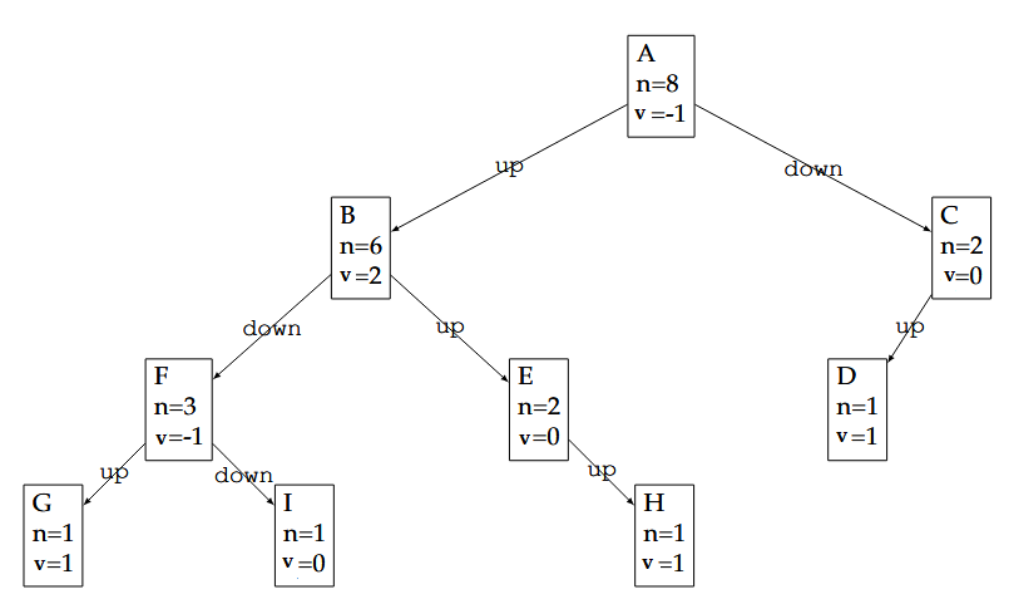
\includegraphics[width=.8\linewidth]{imgs/midterm.7.png}
    \caption{Problem 7: MCTS Tree}
\end{figure}

\textit{Each state has a name (A, B, ..), a return value $v$ and $n$ value. Assume that the constant $c$ in UCB1 is 0.5.}

\subsection*{7.1}

\textit{What is the node that is selected next? Show your work.}

\begin{equation}
    UCB1(s) = \frac{v_i}{n_i}+ c \sqrt{\frac{\ln{N_i}}{n_i}}
\end{equation}

...wherein $v_i$ is our simulation reward for node $s$, $N_i$ is the number of visits of the parent of our node $s$, and $n_i$ is the number of visits for the node $s$.

Let's calculate the UCB1 value for each node in our tree to determine the next state, ignoring our parent node.

\begin{itemize}
    \item \textbf{B} - $\frac{2}{6}+ 0.5 \sqrt{\frac{\ln{8}}{6}} = \frac{1}{3} + 0.5 * 0.589 = 0.333 + 0.294 = 0.627$
    \item \textbf{C} - $\frac{0}{2}+ 0.5 \sqrt{\frac{\ln{8}}{2}} = \frac{0}{2} + 0.5 * 1.02 = 0.501$
    \item \textbf{F} - $\frac{-1}{3}+ 0.5 \sqrt{\frac{\ln{6}}{3}} = \frac{-1}{3} + 0.5 * 0.773 = 0.053$
    \item \textbf{E} - $\frac{0}{2}+ 0.5 \sqrt{\frac{\ln{6}}{2}} = 0.5 * 0.947 = 0.473$
    \item \textbf{D} - $\frac{1}{1}+ 0.5 \sqrt{\frac{\ln{2}}{1}} = 1 + 0.5 * 0.832 = 1.416$
    \item \textbf{G} - $\frac{1}{1}+ 0.5 \sqrt{\frac{\ln{3}}{1}} = 1 + 0.5 * 1.048 = 1.524$
    \item \textbf{I} - $\frac{0}{1}+ 0.5 \sqrt{\frac{\ln{3}}{1}} = 0.5 * 1.048 = 0.524$
    \item \textbf{H} - $\frac{1}{1}+ 0.5 \sqrt{\frac{\ln{2}}{1}} = \frac{-1}{3} + 0.5 * 0.832 = 0.083$
\end{itemize}

Since \textbf{G} has the highest calculated UCB1, we will choose that node.

\subsection*{7.2}

\textit{What action is next for the selected node? This action will make a new state call it “J”.}

There is no specified rule presented - it seems to suggest, by naming, that it chooses the up action first, then later checks the down action. This could also occur in a random choice, which would also work if both actions had equivalent probability in our scenario. For now, we'll assume it's up first based on precedence and move from there.

\subsection*{7.3}

\textit{What is the “n” and “v” value for the new state “J”?}

The new node, unvisited and freshly created, is initialized with $n=0$ and $v=0$.

\subsection*{7.4}

\textit{If the simulation rollout from the expanded node gives a value of 1, backup that value to all of the affected nodes}

Working backwards:

\begin{itemize}
    \item \textbf{J} - $n=1$, $v=1$
    \item \textbf{G} - $n=2$, $v=2$
    \item \textbf{F} - $n=4$, $v=0$
    \item \textbf{B} - $n=7$, $v=3$
    \item \textbf{A} - $n=9$, $v=0$
\end{itemize}

\subsection*{7.5}

\textit{Assume that after this final rollout, we've run out of time to run the MCTS simulation and must now choose an action from state A. What action will be chosen and why if we use the greedy tree policy.}

We would choose the "up" action moving into state \textbf{B} over \textbf{C} as it's current value at this state (3) is higher than 0.



\section*{Problem 8}
\textit{In this question we are comparing mean and variance of the estimate reward for on-policy and off-policy algorithms. Consider the on-policy scenario below where actions are taken under target policy $\pi$:}

\begin{center}
    \begin{tabular}{ |c|c|c| }
        \hline
        Action        & Reward & Probability via $\pi$ \\
        \hline
        $\rightarrow$ & +10    & 0.9                   \\
        \hline
        $\leftarrow$  & +20    & 0.1                   \\
        \hline
    \end{tabular}
\end{center}

\subsection*{8.1}

\textit{What is the expected value (mean) of estimated reward?}

The expected value of our estimated reward is the sum of the total rewards multiplied by the probability of each action. Thus:

\begin{equation}
    \sum \pi(a) * r_a
\end{equation}

\begin{equation}
    (0.9 * 10) + (0.1* 20) = 11
\end{equation}

\subsection*{8.2}

\textit{What is the variance of the estimate reward? Hint: use the equation $Var[X] = E[X^2] - E[X]^2$}

\begin{equation}
    E[X^2] = (0.9 * 10^2) + (0.1*20^2) = (0.9*100) + (0.1*400) = 130
\end{equation}

\begin{equation}
    Var[X] = 130 - 11^2 = 130 - 121 = 9
\end{equation}

\subsection*{8.3}

\textit{Now assume that there is a behavior policy that is taking actions with following distribution:}

\begin{center}
    \begin{tabular}{ |c|c|c|c| }
        \hline
        Action        & Reward & $\pi_t$ & $\pi_b$ \\
        \hline
        $\rightarrow$ & +10    & 0.9     & 0.5     \\
        \hline
        $\leftarrow$  & +20    & 0.1     & 0.5     \\
        \hline
    \end{tabular}
\end{center}

\textit{Assume that we don't know the distribution of the target policy and we only know the ratio $\frac{\pi}{b}$ (importance sampling ratio). Numerically calculate the expected reward assuming that the action are taken by the behavior policy.}


\begin{equation}
    (0.5 * 10) + (0.5* 20) = 15
\end{equation}

\subsection*{8.4}

\textit{Calculate the variance of the expected reward?}

Using $Var[X] = E[X^2] - E[X]^2$ again:

\begin{equation}
    E[X^2] = (0.4 * 10^2) + (0.1*20^2) = (0.5*100) + (0.5*400) = 250
\end{equation}

\begin{equation}
    Var[X] = 250 - 15^2 = 250 - 225 = 25
\end{equation}

\subsection*{8.5}

\textit{What is the intuition behind higher variance in off-policy in this example? Can you explain how the importance sampling could increase the variance in off-policy learning?}


In off-policy learning, the behavior policy is used to generate samples for its exploration and the target policy is derived from those samples. The behavior policy may as a result take actions that the target policy would not, leading to our observed difference in the probability distributions of actions for the target and behavior policies. This difference in distribution can cause the importance sampling ratio to be high, leading to high variance in the estimates. On-policy learning (like our first example) has a lower variance as it is more likely to result in the same actions being chosen repeatedly - which would explain the higher probability of choosing a singular action.

\end{document}